\documentclass[border=2pt]{standalone}
\usepackage{tikz}
\usetikzlibrary{decorations.pathmorphing}

\begin{document}

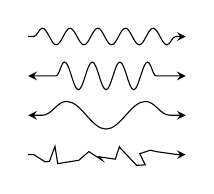
\begin{tikzpicture}
	
	\draw[-stealth,decorate,decoration={snake,amplitude=3pt,pre length=2pt,post length=2pt}] (0,-0.5) -- (2,-0.5);
	
	\draw[stealth-stealth,decorate,decoration={snake,amplitude=5pt,pre length=10pt,post length=10pt}] (0,-1.0) -- ++(2,0);
	
	\draw[stealth-stealth,decorate,decoration={snake,amplitude=5pt,pre length=5pt,post length=5pt, segment length=10mm}] (0,-1.5) -- ++(2,0);
	
	\draw[-stealth,decorate,decoration={random steps,segment length=3pt,amplitude=4pt,pre length=2pt,post length=3pt}] (0,-2) -- ++(2,0);
\end{tikzpicture}

\end{document}
